\documentclass[UTF8,a4paper]{ctexart}
%\documentclass[a4paper]{article}
%\usepackage{ctex}
\usepackage{underscore}
\usepackage{multicol}
\usepackage{graphicx}
\usepackage{listings}
\usepackage{amsmath,amssymb,amsfonts}
%\usepackage{url}
\usepackage[colorlinks,linkcolor=blue]{hyperref}
\title{周报}
\author{LiuYan}
\date{\today}
\begin{document}
\section{2019.07.10}
\subsection{Search domain of K}
find a stable pi controller box using interval analysis, then it's possible to find a stable pid controller box in the same way. The box is the search domain of K.
\begin{itemize}
\item (examples/lab7.cpp)the stable pi controller box: depict by vibes(no data but can see subject number:([-100,-10],[-10,0]))\\
\item (examples/in1.cpp)the stable pi controller box: Box after HC4:([-100, -13.66056572379367] ; [-26.74742268041238, 0])\\
\item (examples/in2.cpp)using HC4 to find stable PID controller box: "x before HC4:([-100, 0] ; [-100, 0] ; [0, 100])
 Box after HC4:([-100, -13.45070422535211] ; [-26.77559912854032, 0] ; [0, 20.44925124792014])"
\\
\item choose search domain:([-100,-12],[-27,0],[0,21])
\end{itemize}
%\paragraph{验证}
%by matlab simulation,choose K=(-50,-20,15), the closed-loop system is stable.\\
理解全局最优:由于初始搜索域并不是整个空间,所以不完全是全局最优的。要求:如果要在整个空间寻找全局最优,对计算机计算能力和内存要求过高。
\paragraph{结果}
iter=3117,  size_heap=0,  ymax=44.4284,  uplo= 44.7585\\
iter=3117,  size_heap=0,  ymax=44.4284,  uplo= 44.7585\\
 best bound in: [44.7585,44.8771]\\
 Relative precision obtained on objective function: 0.00264479  [passed]  0.01\\
 Absolute precision obtained on objective function: 0.118691  [failed]  0\\
 precision on variable domains obtained 0.0001  uplo_of_epsboxes 44.7585\\
 best feasible point (-19.7028 ; -0.002648 ; 1.02108)\\
 cpu time used 56.48s.\\
 仿真结果:不稳定,输出y在70s内即发散为脉冲信号。
 \paragraph{扩大搜索域}
 当扩大搜索域为([-100,100],[-100,100],[-100,100]),6分钟后得到best feasible point (50.4389 ; -82.9962 ; -84.8925),仿真依旧不稳定。
 \subsection{PI控制器}
 1.已确定搜索域为([-100, -13.66056572379367] ; [-26.74742268041238, 0]);[0,0].\\
 2.iter=7516,  size_heap=0,  ymax=39.7503,  uplo= 40.1368\\
iter=7516,  size_heap=0,  ymax=39.7503,  uplo= 40.1368\\
 best bound in: [40.1368,40.1518]\\
 Relative precision obtained on objective function: 0.000372783  [passed]  0.01\\
 Absolute precision obtained on objective function: 0.0149679  [failed]  0\\
 best feasible point (-58.7091 ; -3.46578 ; 0)\\
 cpu time used 36.78s.\\
 仿真结果:依旧不稳定。\\
 分析:劳斯判据有问题\\
 \subsection{检查}
 对于特征多项式$a5*s^5+a4*s^4+a3*s^3+a2*s^2+a1*s+a0=0$\\
  \paragraph{wrong routh vector}
  错误的劳斯相量如下:
  \begin{lstlisting}[language={[ANSI]C},numbers=left,numberstyle=\tiny]  
  b1=(a4*a3-a5*a2)/a4;
b2=(a4*a1-a5*a0)/a4;
b3=0;
c1=(b1*a2-a4*b2)/b1;
c2=(b1*a0-a4*b3)/b1;
d1=(c1*b2-b1*c2)/c1;
r1=[a5;a4;b1;c1;d1];
   \end{lstlisting}
    \paragraph{right routh vector}
  由于特征多项式最高次数为n=5次方,所以对应的劳斯相量应该有n+1=6个元素如下:
    \begin{lstlisting}[language={[ANSI]C},numbers=left,numberstyle=\tiny]  
  b1=(a4*a3-a5*a2)/a4;
b2=(a4*a1-a5*a0)/a4;
b3=0;
c1=(b1*a2-a4*b2)/b1;
c2=(b1*a0-a4*b3)/b1;
d1=(c1*b2-b1*c2)/c1;
e1=a0
r1=[a5;a4;b1;c1;d1;e1];
   \end{lstlisting}
   \subsection{PI控制器结果}
   \begin{figure}
  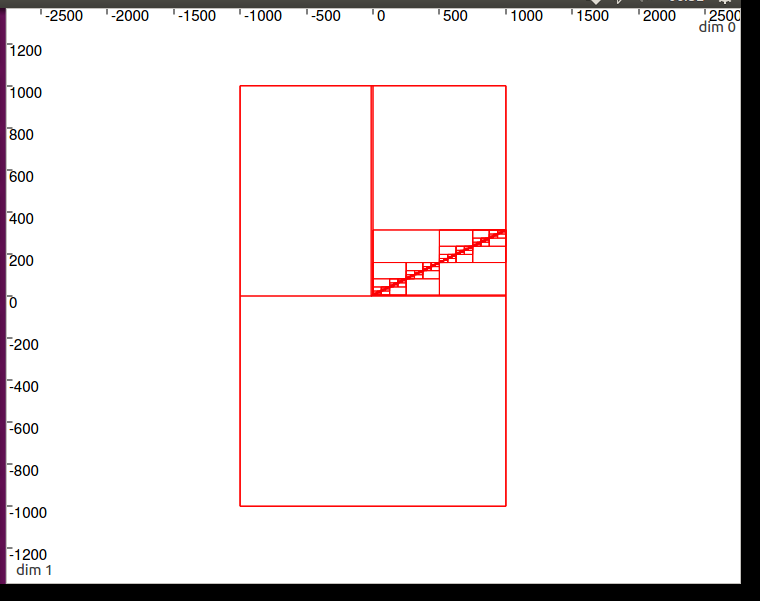
\includegraphics[width=.8\linewidth]{1.png}
  \caption{PI控制器:在([-1000,1000],[-1000,1000])内均无解}
  \label{fig:boat1}
\end{figure}
 \begin{lstlisting}[language={[ANSI]C},numbers=left,numberstyle=\tiny] 
iter=34924,  size_heap=17417,  ymax=8.96088e-317,  uplo= 35.0901
time limit 360s. reached 
 best bound in: [35.0901,inf]
 Relative precision obtained on objective function: inf  [failed]  0.01
 Absolute precision obtained on objective function: inf  [failed]  0
 precision on variable domains obtained 0.0001  uplo_of_epsboxes 36.2078
 no feasible point found 
 cpu time used 360.012s.
\end{lstlisting}
 \subsection{PID控制器结果}
 \begin{lstlisting}[language={[ANSI]C},numbers=left,numberstyle=\tiny]
 iter=1770019,  size_heap=439808,  ymax=6.42317e-317,  uplo= 35.3004
time limit 36000s. reached 
 best bound in: [35.3004,inf]
 Relative precision obtained on objective function: inf  [failed]  0.01
 Absolute precision obtained on objective function: inf  [failed]  0
 precision on variable domains obtained 0.0001  uplo_of_epsboxes 35.3004
 no feasible point found 
 cpu time used 36000s.
\end{lstlisting}
\section{水下机器人建模与鲁棒控制—杨睿}
控制:
\begin{itemize}
\item 被控对象:四自由度(横荡,纵荡,垂荡,艏摇)模型。 鲁棒控制器:艏摇模型。
\end{itemize}
\paragraph{水下航行器定位与制图的卡尔曼与区间方法比较}
在本文中,我们使用卡尔曼滤波器和鲁棒状态观测器来比较水下航行器的定位和映射,使用车辆和位于海底的一组信标之间的仅范围测量。 正如预期的那样,我们表明当我们拥有关于车辆位置和信标的相当好的先验信息时,卡尔曼滤波器表现很好。 基于集合隶属度方法,鲁棒状态观测器证明了在存在异常值的情况下以非常粗略的精度为代价提供一致估计(其中真实解决方案在估计置信域中)的出色能力。 将讨论这种缺乏精确度的根源。
\paragraph{Fuzzy Matrix Contractor Based Approach for Localization of Robots}定位包括找到一些机器人相对于其位置和方向的姿势。 在一组机器人在平面表面上定位的情况下,每个机器人使用可以根据矩阵方程考虑的约束与其他机器人链接。 因此,本章讨论了使用与模糊矩阵承包商相关的角度和距离约束的机器人组的定位。 基于方位距离和方位距离约束的矩阵承包商有助于通过一组机器人有效传播模糊不确定性,以便在没有绝对帧时进行定位。 最后,各种机器人小组已被考虑用于验证拟议的承包商即。 方位角,距离,方位距离和承载距离承包商使用高斯模糊不确定性.\\
\section{2019.07.15}
\section{chapter: Comparison of Kalman and Interval
Approaches for the Simultaneous
Localization and Mapping
of an Underwater Vehicle}
Simultaneous Localization and Mapping 同时定位与地图创建(SLAM)\\
confidence 置信度\\
a fiber optic gyroscope inertial navigation system光纤陀螺惯性导航系统
\begin{itemize}
\item problem: Simultaneous estimate the pose of the vehicle and building the map of its environment.
\item solution: SLAM for localization, 
\end{itemize}
在给水下仪器周围环境建模时估计该仪器姿态时,如何实现两者的同时性是个问题。定位和地图其中一者越精确,另一者也会越精确。对于定位,在水下用SLAM代替GPS进行定位。可以在仪器航行时实时定位。甚至不用先验知识,获得的数据可以直接用于在线校准,节省了时间。SLAM需要对环境进行感知,工具可以是相机,声纳或者其他传感器。本章只讨论声学传感器。(总分为定位和构建地图,引出定位问题为状态估计问题)\\

这种类型的状态估计问题通常用卡尔曼滤波器来求解,因为它是一个经过研究充分,易于理解的状态估计器,已成功用于许多定位问题和SLAM问题。虽然当仪器与信标的初始状态估计良好时,这种方法非常有效,但是当系统没有良好的条件,当出现非线性且得不到良好的初始状态估计时,它的性能会变差。所以卡尔曼滤波器在这些情况下可能会产生高置信度的差估计,并且拒绝较好值得测量,无法将他们和奇异值区分开来,使得检测故障变得棘手。本文提出一种新的集合论方法和卡尔曼滤波器进行比较。集合理论是概率不可知的,有些适用于奇异值有鲁棒性的非线性系统。参考文献8用海上定位比较了卡尔曼滤波器和区间方法。(指出卡尔曼估计的不足)\\

本文比较了并综合了集合论和概率方法去求解水下机器人的SLAM问题。水下定位主要依赖于声音传播的时间为我们提供一些关于水下机器人和一些海标之间的距离。此时集合论方法比较有吸引力。(本文的主要内容)\\

本文组织结构如下。8.2为系统和传感器建模,并考虑了不确定性。8.3将问题描述为一个概率状态估计问题,并用卡尔曼滤波器求解。8.4回忆了区间状态估计的规则和它的优缺点。8.5用真实的数据集合比较了这两种方法。8.6分析了结果,特别讨论了区间估计器缺乏精度的原因。8.7总结本文。\\
\section{2019.08.02}
Matlab的符号运算有所限制,改用Mathematica,需先了解Wolfram语言。
\subsection{Wolfram}
\paragraph{入门}在mathematica的实际操作中,记住三个秘诀即可完成绝大部分功能:\\
1.内置指令首字母大写,采用驼峰原则;\\
2.函数的参数均使用[];\\
3.列表用于储存范围等,使用{};
\paragraph{wolfram语法}
\begin{itemize}
\item $\pi$: Pi
\item $e$: E
\item $A*B$: Dot[A,B]
\end{itemize}
\section{2019.08.06}
\subsection{程序并发,多线程}
1.并行编译: make -j4 file1 file2 file3 file4\\
2.并行运行: 
std::this_thread::sleep_for: 表示当前线程休眠一段时间,休眠期间不与其他线程竞争CPU,根据线程需求,等待若干时间\\
1.我们需要数据并行: 是在数据方面——每个线程在
不同的数据部分上执行相同的操作(第二种方式),被称为数据并行(data
parallelism)\\
2.共享数据
3.互斥锁
4.时间开销项:链接库,
5.多线程需要修改makefile文件为:\\
 \begin{lstlisting}[language={[ANSI]C},numbers=left,numberstyle=\tiny]  
CXXFLAGS += -pthread -fPIC $(COMMON_FLAGS) $(WARNINGS) -std=c++11
NVCCFLAGS += -D_FORCE_INLINES -ccbin=$(CXX) -Xcompiler -fPIC $(COMMON_FLAGS) -std=c++11
LINKFLAGS += -pthread -fPIC $(COMMON_FLAGS) $(WARNINGS) -std=c++11
   \end{lstlisting}
   6.管理线程的函数和类在 <thread> 中声明,而保护共享数据的函数和类在其他头文件中声
明。\\
7.由于线程是有生命周期的,所以须在对象销毁之前就去访问数据,不然单线程一结束,局部对象也会被销毁。thread中的类函数join函数可以确保局部变量在线程结束之后才被销毁。\\
\section{2019.08.07}
\href{http://www.xuetangx.com/courses/course-v1:TsinghuaX+20740084X+2019_T1/about}{《基于linux的c++》}
\paragraph{源代码排版}
\begin{itemize}
\item 递进层次应使用左缩进格式
\item 每行代码不能过长,不能超过 $80$ 个字符
\item 函数代码不超过 $60$ 行
\item 使用空行区分不同功能代码
\item 复合语句书写格式要统一
\item 除非特别必要,否则不要在一行上写多条语句
\item 命名规范要一致
\item 无论采用什么标准,都一定要一直按照该标准进行代码的编辑
\end{itemize}
\section{2019.08.08}
1.普通用户不能添加新的用户,不能删除其他用户的配置文件。
2.如何设置私人文件为他人不可读?  设置文件权限
3.sudo之后的普通用户可以修改所有用户的密码。(很危险)
4..bash_history文件只有本用户和root可读。
5.如何给普通用户加上sudo权限。
\paragraph{iomanip.h}
\section{2019.08.09}
\paragraph{Introduction \& 基于区间分析的结构化 $H_\infty$ 鲁棒综合控制器}
1.读老师和师兄毕业论文,了解前言基本架构2019-08-09\\
2.收集领域内发展概况,理清逻辑线2019-08-10\\
3.书写前言2019-08-12\\
4.修改并上交2019-08-13\\
\paragraph{水下机器人鲁棒控制研究批注}
研究背景及意义:海洋强国战略,水下机器人探索和开发海洋,水下机器人介绍和分类,其中AUV最好,本文干嘛了,鲁棒性,实时性要求FPGA适用于浮点数矩阵运算,MOOS仿真减少潜在的损失。\\
研究现状:对比了各种控制方法,鲁棒控制优势,本文主要工作流程。\\
\section{2019.08.10-08.11}
\paragraph{函数}
cpp编辑顺序: 函数声明,主函数,函数定义。\\
值传递机制:
\begin{itemize}
\item 形式参数再函数调用时才分配存储空间,并接受实际参数的值。\\
\item 实际参数可以是复杂的表达式,在函数调用前被计算\\
\item 形参和实参可同名\\
\item 形参和实参必须保持数目,类型和顺序的一致\\
\item 值得复制过程单向不可逆,函数内部对形参得改变不会反应到实参。\\
\end{itemize}
算法中做循环运算时,一定要避免不必要的重复运算,否则会降低算法效率。\\
递归:递推 $+$ 回归\\
不要在头文件中定义全局变量。\\
static使得量具有静态(局部)生存期,下一次进入到该语句块时会使用上一次退出时的值(有记忆性)\\
%\section{2019.08.10-08.11}
%\newpage
%\subsection{绪论}
%\subsubsection{课题背景与研究意义}
%作为一个蕴含丰富水资源的星球,地球面积的百分之七十一被海洋覆盖。丰富的石油和天然气资源以及其他潜在资源使得海洋地球科学领域的海洋探测和开发活动生生不息,在这样的环境下,海洋探测技术和设备也日益进步,衍生了一系列的水下机器人系统。 这些水下机器人系统包括:有缆遥控水下机器人(Remotely Operating Vehicle, ROV)和自主式水下机器人(Autonomous Underwater Vehicle, AUV) 干预式自主水下机器人(Intervention Autonomous Underwater Vehicle, IAUV), 无人船(Autonomous Surface Craft, ASC), 水下滑翔机 (Underwater Glider, UG) \cite{}。其中自主式水下机器人(AUV)由于其高度的自主性,造价成本低,作业环境要求低的特点,广泛用于海洋探测和开发。
% ref1th_3th: 自主式水下机器人(AUV) AQUA EXPLORER 2 (AE2)自1997年首次发射后进行了三次海上试验和五次电缆检查任务,检查电缆总长度超过400公里。\cite{}
%ref1th_197th: 2012年东北大学的张磊等人利用自主式水下机器人(AUV)声纳实测数据成功实现了海底三维环境的重构\cite{}。 
%ref1th_175th: 2015年华中科技大学的向先波等人利用自主式水下机器人(AUV)携带智能采样器进行水下采样作业\cite{}。
% ref1th_6th: 挪威奥斯陆大学的Ann Elisabeth Albright Blomberg等人利用水下机器人针对不同的海底环境进行试验,验证了AUV探测和监测海洋气体渗漏的能力\cite{}。
%  ref1th_96th:  历时三年的“caddi - cognitive Autonomous Diving Buddy”FP7项目研发了$4$ 台水下机器人:MedusaS,PladyPos, BUDDY,R2。其中BUDDY,R2为自主式水下机器人(AUV), 在2016年发布的视频中它们做到了监测潜水员的姿势和手势识别,以及完成了极限搜索任务\cite{}。
% newref_1: 在过去的15年里,自主式水下航行器(auv)为海洋地质学家们提供了高分辨率的海底绘测数据,从极端的海底热液喷口到极低冰盖,AUV的海底成像能力都十分有效\cite{}。
%ref3th: IAUV作为AUV的一个分支,主要干预石油和天然气开发,海上搜救,深海考古,永久海洋观测平台的维修等活动。目前存在的IAUV仅有:ALIVE, SAUVIM and GIRONA 500,它们一般会配备机械手,
%可以实现的最简单的操作为插拔阀门,旋转阀门,以及回收自由浮体等\cite{}。
%
%虽然已经有许多 AUV 被生产出来并投入工作,但是面对复杂且时刻变化的海洋环境,保持 AUV 的高度自主性和稳定性仍具有很大的挑战。想要实现对 AUV 的精准控制效果, 我们迫切需要找到一个控制律实现 AUV 各个自由度上运动的控制。
%
%newref_4: 比起未建模控制,基于模型的控制系统往往更加有效\cite{},中国海洋大学的杨通过水动力建模与鲁棒控制验证了“CISCREA”水下机器人模型的有效性\cite{}。
%Robust-control-of-uncertain-systems--Classical-results-and-rece_2014_Automat: 从控制角度而言,水下机器人模型是一个不确定系统,它的不确定性主要分为两部分: 非结构不确定性和结构不确定性\cite{}。
%非结构不确定性常常来源于未建模动态,由于本文基于杨的精确建模方案,所以不需要考虑非结构不确定性。结构不确定性(参数不确定性)主要源于模型内部的不确定的参数,例如系统不精确建模产生的不确定系数、系统作业时AUV配件变化带来的参数的变化。具体在于当AUV架上一台相机时,引起的质量改变会使得模型转动惯量参数发生变化,经典的控制方法可能不再起精准快速的控制效果。为了应对实际需求,我们需要设计一个考虑参数不确定性的鲁棒控制器。
%
%鲁棒控制理论中3种主要方法综述_二_汤伟:由于AUV模型是一个六自由度的多入多出(Multiple Input Multiple Output, MIMO)模型,而$H_\infty$鲁棒控制综合刚好是为具有模型摄动的 MIMO 系统设计的频域控制方法\cite{}。
%ref_5th, Fixed-Order-H--Controller-Design-for-Systems-with-Pol_2011_IFAC-Proceedings:过去已有的案例中,其中有为多项式不确定性系统设计定阶的 $H_\infty$ 鲁棒控制器\cite{} 和降阶鲁棒控制器\cite{},由于控制器参数是决策变量,所以可以考虑PID等更加一般化的控制器结构。结构简单的定阶和降阶控制器适应了 AUV 近年来的硬件发展趋势,越来越多的 AUV 运行在嵌入式系统上。而嵌入式系统有限的计算能力正好需要结构精简的定阶和降阶控制器。
%\subsubsection{研究现状}
%review_robustcontrol_uncertainparameter: 现代鲁棒控制主要为两个大分支: $H_\infty$ 最优控制和参数不确定性下的鲁棒控制\cite{}。1978年 Kharitonov 定理将鲁棒控制引向参数不确定性的鲁棒控制,而 1989年 Doyel等人提出的 DGKF 方法(Ricatti 方程)求解出了$H_\infty$ 控制控制器。后来1994年 Apkarian 等人提出了线性矩阵不等式(Linear Matrix inequality, LMI)方法将 $H_\infty$ 鲁棒控制问题转化为一个凸优化问题,问题的目标函数是线性分式变换(Linear Fractional Transformation, LFT)的 $H_\infty$ 范数,约束条件为鲁棒稳定性条件。
%从而可以计算出一个局部最优的控制器状态空间表达参数\cite{}。然而无论是 Ricatti方程还是 LMI方法都只是求解了局部优化问题,且在综合问题的求解过程中不考虑广义控制器结构和非凸约束。
%ref14th-20th: 因此,区间分析理论为非凸优化问题发展了以极小极大分支定界算法为代表的全局优化方法。
%
%ref17th: 1966年 Moore 提出了实数区间(和区间向量)与实数区间计算方法的概念,区间算法被设计成在计算过程中自动对初始数据中累积的舍入误差、近似误差和传播的不确定性提供严格的界限。它的实际应用领域包括化学和结构工程、经济学、控制电路设计、光束物理学、全局优化、约束满足、小行星轨道、机器人、信号处理、计算机图形学和行为生态学。区间分析允许我们计算积分的精确值的区间包围。区间方法可以用不精确的数据来约束线性系统的解。对于全局优化、约束满足和参数估计问题,存在严格的区间分枝定界方法\cite{}。 为后来出现的极小极大化区间分支定界算法奠定了基础。
%ref14th: 2001年 Jaulin 发表的区间分析应用,在原有的区间理论的基础上,提出了inclusion function 和 contractor 等重要概念。inclusion function 完成了区间向量之间映射的包含运算,contractor 有效地利用一系列数学迭代方法求解了条件约束问题(Constraint Satisfaction Problem, CSP),在一定精度下得到了包裹问题真实解的可靠的区间向量\cite{}。
%ref15th: 当 CSP 的变量是实数集的子集时,引入集区间(称为i集)后可使用约束传播方法构建 contractor 求出 CSP 解的包围\cite{}。约束传播方法是求解非线性非凸问题的一种常用方法,它可以有效地解决未知变量属于离散集或当这些变量是实数集的向量时的非线性非凸问题。区间分析自提出后被用来解决了许多实际问题,例如paper_seppath: 路径规划, state_e: 状态估计等。
%ref16th: 超过100公里的无人船导航应用也验证了区间分析的有效性\cite{}。
%
%ibex: 在区间分析广泛应用的同时,与之相关的IBEX项目在2007年开始启动。IBEX是一个用于实数约束处理的开源c++库。它为处理非线性约束提供了可靠的算法。特别地,舍入误差也被考虑在内。它基于区间算法和仿射算法。Ibex的主要特性是它能够通过 contractor 编程范式声明性地构建策略。它也可以用作黑盒求解器。可以解决的两个象征性问题是: 系统求解计算了(非线性)方程组各解的包络形式。全局优化利用目标极小值的保界,计算了非线性约束下某函数的全局极小化问题\cite{}。该全局优化黑盒为后来的极小极大分支定界算法立下了基础。
%
%ref20th: Clement 结合区间分析技术和凸优化求解了鲁棒约束可行性问题(Robust Constraint Feasible Problem, RACFP),加快了问题求解速度。但是求得的局部解不能证明是全局最优的\cite{}。
%ref18th: 2014年  Ninin 等人将仿射算法嵌入到基于区间分析的经典分支定界算法中,解决了一部分的标准全局优化问题\cite{}。
%ref21th: 2015年  Dominique等人利用分支定界算法(IBBA) 证明了针对一个特定的 $H_\infty$ 鲁棒控制问题, 它的解控制器的存在与否性。
%ref19th: Dominique等人提出了MMIBBA算法,将结构化的$H_\infty$ 鲁棒控制综合问题转化成一个求极小极大值的全局优化问题后,用MMIBBA算法为“CISCREA”水下机器人求得了一个全局最优的PID控制器。
%实际上,MMIBBA是一种创新的综合结构控制器H约束、稳定性约束和参数不确定性的全局优化方法。MMIBBA首先从理论上证明了控制器存在,其次,其结果得到了精确的保证。尽管有这些优点,MMIBBA打开了讨论高度一般化的结构和约束设计问题的挑战。H结构和约束设计对优化结果影响很大。
%%Robust-control-of-uncertain-systems--Classical-results-and-rece_2014_Automat: 
%%\paragraph{1.水下机器人在海洋探测与开发活动中扮演着不可或缺的角色。[]}
%%\begin{itemize}
%%\item 人类近年来对海洋的探索与开发得益于日益进步的海洋探测技术和设备,在这些水下设备中,水下机器人扮演着十分重要的角色。
%%\item ref1th: 模糊逻辑控制,有着控制结构简单,易于设计,较高的成本效益等优点,广泛用于水下机器人的制导与控制。
%%\item ref1th_197th: 2012年东北大学的张磊等人利用水下机器人声纳实测数据进行海底三维环境的重构。 ref1th_175th: 2015年华中科技大学的向先波等人利用水下机器人携带智能采样器进行水下采样作业。 ref1th_6th 挪威奥斯陆大学的Ann Elisabeth Albright Blomberg等人利用水下机器人针对不同的海底环境进行试验,验证了探测和监测海洋气体渗漏的能力。ref1th_3th AQUA EXPLORER 2 (AE2)是世界上第一个也是唯一一个能够自主跟踪水下电缆并测量其埋深的水下机器人,海底管道和电缆跟踪检查。自1997年首次发射以来,AE2已经进行了三次海上试验和五次电缆检查任务。检查电缆总长度超过400公里。1999年,在对一根穿越台湾海峡的海底通信电缆的实际检测中,证明AE2对水流和沙波具有较强的抗冲击能力。ref1th_96th  历时三年的“caddi - cognitive Autonomous Diving Buddy”FP7项目研发的协作水下机器人系统做到了监测和帮助潜水员的水下作业,重点在哪里放置在潜水员的模型的三维重建(姿势估计和识别的手势)通过远程和本地传感技术,从而使行为解释;了解潜水员,目的是解释潜水员的模型和生理测量,以确定潜水员的状态;以及多机器人协作与控制,旨在研究潜水员与具有丰富感觉运动技能的潜水器之间的交互作用,重点是与作为整体车-潜水员编队组成部分的潜水员进行协作控制和优化编队。(基础的CADDY水面机器人MedusaS, 备用的CADDY水下机器人PladyPos,极限搜索, BUDDY auv 识别手势, R2 备用水下机器人,) ref1th_13th 中通过映射流场研究AUV受环境流的影响,从而改善AUV导航性能。
%%\item 2018年4月,我国自主研发的“海燕”深海水下滑翔机首潜8213米 刷新世界纪录。虽然水下滑翔机的航行速度较慢,但其制造成本和维护费用低、可重复使用、并可大量投放等特点,缺点是其航迹控制和定位精度低,航速慢,在风浪较大的海面可能会出现随波逐流的情况。 ref1th_194th利用水下滑翔机进行水下采样作业。
%%\item ref3th: 水下机器人参与的活动有永久水下天文台的维修,海底油井、电缆传感器网络、管道和海底栖生物站的部署和回收。ALIVE, SAUVIM and GIRONA 500具有自主干预能力。1)阀门转向及连接器对接至水下面板时堵/拔堵;(2)自由浮阀转向,演示学习;(3)多用途自由浮体回收。这些机器人干预活动包括: 石油和天然气开发,海上搜救,深海考古,永久海洋观测平台.
%%\item ref2th: 水下机器人系统包括:有缆遥控水下机器人(Remotely Operating Vehicle, ROV)和自主式水下机器人(Autonomous Underwater Vehicle, AUV) 干预式自主水下机器人(Intervention Autonomous Underwater Vehicle, IAUV), 无人船(Autonomous Surface Craft, ASC), 滑翔机系统 (Gliders system, GS)。
%%\item newref_1: 自主水下航行器(auv)在海洋地球科学领域有着广泛的应用,并越来越多地应用于科学、军事、商业和政策领域。它们能够自主地操纵宿主船,这使得它们非常适合探索极端环境,从世界上最深的热液喷口到极地冰盖下。它们彻底改变了我们对海底成像的能力,提供了比水面船只更高分辨率的海底测绘数据,尤其是在深水中。这项工作的重点是AUV数据在海洋地球科学方面取得的重大进展。主应用程序i)海底火山活动、深海热液喷口研究ii)映射和监测低温流体逃脱特性和化学合成的生态系统,3)底栖生物栖息地映射在浅,深水环境中,海底和iv)映射的形态学特征(如生成bedforms下冰或沉积物重力流)。提出了一系列新的数据集,突出海洋地球科学研究越来越多功能性的水下机器人,包括我)多频声成像的拖网影响深水珊瑚成堆,iii)的高分辨率海底photomosaics深海深处,活跃的潜艇和iii)速度测量密度流。未来与海洋地球科学潜在相关的AUV技术的发展包括具有增强悬停、长续航能力、极深或快速响应能力的新车辆,而新传感器的发展将进一步扩大可测量的地球化学参数的范围。(海底测绘和监测)
%%\item newref_2: 三次水下机器人在运动中表现出更多的自由度。特别是,他们可以悬停并进入复杂的水下空间
%%\end{itemize}
%%\paragraph{2.对AUV性能的要求,参数不确定性限制AUV的性能。需要鲁棒控制[]}
%%虽然已经有许多 AUV 被生产出来并投入工作,但是面对复杂且时刻变化的海洋环境,保持 AUV 的高度自主性和稳定性仍具有很大的挑战。想要实现对 AUV 的精准控制效果, 我们迫切需要找到一个控制律实现 AUV 各个自由度上运动的控制。
\section{2018.08.16}
\paragraph{title: The Cubli: A Cube that can Jump Up and Balance. author: Mohanarajah Gajamohan. year: 2012}
%progressive ralationship
关键词:Inverted pendulum system, Cubli.\\
Cubli介绍:The Cubli is the small cube which can jump up from a resting position without external support.
The Cubli jumps up by stopping the momentum wheels which rotate at high angular velocities.
When the cubli arrived the stand-up position, it will keeps the balance on a corner because of the controller motor torques.\\
%problem 1: How to build the cubli?\\
%This paper present the concept of three dimensional Cubli along with the development of the one dimensional design, modeling, identification and control.
%The paper also present a control process to eliminate the sensor offsets during balance maneuver.\\
%progressive relationship
文章内容:one dimension prototype, estimation and control \\
%The prototype consists with the square plastic plate which holds the momentum exchange wheels through the motor on its center and the braking mechanism on its corner.
My question:
\begin{itemize}
\item 最后动量交换轮是停下来了吗? 没有,动量轮在和摆体碰撞之后,和摆体一起运动(相同的速度,相对于摆体静止),快到达站立位置时,电机输出电流产生力矩,使得摆体和动量轮又开始速度分离,最终摆体静止达到平衡,动量轮以一定速度转动。
\item 改变动量交换轮质量 $m_w$ 会改变 $I_w$, 但是 $I_w$ 是经过实验辨识(固定摆体,给动量交换轮上电机驱动,测角速度: $I_{w} \ddot{\theta}_{w}(t)=K_{m} u(t)-C_{w} \dot{\theta}_{w}(t)$)出来的,所以怎么设置不确定性参数? 不确定性来自于外部风浪流,而不是模型不确定性。
\item 关于本文复现工作。第一步,不考虑偏移量进行MATLAB仿真,LQR控制器作用下,以 $(-0.1, 2, 2)$ 为初始状态,最终状态为(0, 0, 0),可以看出最终动量交换轮的速度为 $0$,与稳定系统性质一致(在输入为零时,系统可以由任何状态趋近于0)。但是论文上认为动量交换轮最终是会匀速转动的,为什么?\\
判断一:仿真结果无误。\\
\end{itemize}
conclusion: LQR controller was designed to balance the one dimension Cubli prototype after it jump up to the stand-up position. A control process is also presented to eliminate the sensor offsets during balance maneuver.
%\paragraph{刚体转动定律: 为研究一维原型的物理规律,进行肌理建模}
\section{2019.08.17}
\paragraph{处理不确定性}
one dimension Cubli prototype model:\\
$\begin{aligned} \ddot{\theta}_{b}=& \frac{\left(m_{b} l_{b}+m_{w} l\right) g \sin \theta_{b}-T_{m}-C_{b} \dot{\theta}_{b}+C_{w} \dot{\theta}_{w}}{I_{b}+m_{w} l^{2}} \\ \ddot{\theta}_{w}=& \frac{\left(I_{b}+I_{w}+m_{w} l^{2}\right)\left(T_{m}-C_{w} \dot{\theta}_{w}\right)}{I_{w}\left(I_{b}+m_{w} l^{2}\right)} \\ &-\frac{\left(m_{b} l_{b}+m_{w} l\right) g \sin \theta_{b}-C_{b} \dot{\theta}_{b}}{\left(I_{b}+m_{w} l^{2}\right)} \end{aligned}$\\
%可能的不确定参数p: $-\frac{\sqrt{2}}{2} < \sin \theta_b < \frac{\sqrt{2}}{2}$  ($-0.707 < \sin \theta_b < 0.707$)
线性化:$\sin\theta_b \approx \theta_b$
\paragraph{c++}
在头文件包含标准库,之后被其他函数包含之后就可以用该标准库;否则标准库的作用域仅仅限于本文件。\\
\section{2019.08.19}
\subsection{不确定性建模}
%\paragraph{title:  author: year:}
\paragraph{title: Robust control of uncertain systems: Classical results and
recent developments. author: Ian R. Petersen. year: 2014}
关键词: 不确定性建模\\
%the plant   a set of systems
Consider the linear system, the plant to be controlled can be described via the state space model.
\begin{itemize}
\item parametric uncertainty
\item linear fractional transformation uncertainty (can interpret the nonlinear time-vary dynamic uncertainty)
\end{itemize}
\subsection{细节}
%真上确界和真下确界
1. Essential supremum and infimum \\
The $H_\infty$ norm of the $c \times r$ matrix transfer function $M(s)$ is: 
\begin{equation}
\|M(s)\|_{\infty} \doteq \operatorname{ess} \sup _{\omega \in \mathbb{R}} \overline{\sigma}(M(j \omega))
\end{equation}
the essential supremum of the greatest singular value of $M(j \omega)$ in frequency domain.
% ess sup的定义请看 d:\papers\帮助文档
\paragraph{title: Saturation based nonlinear PID control for underwater vehicles: Design,
stability analysis and experiments.  author: J. Guerrero a, J. Torres a, V. Creuze b, A. Chemori b, E. Campos c.  year: 2019}
This paper proposed to design a controller for trajectory tracking in depth and yaw dynamics. The controller improved the robustness through replace the constant feedback gains with the whole nonlinear function, and improved nonlinear saturate control law.\\
结论:This paper designed a control law without considering the coupling relationship between the degrees.\\
\section{2019.08.20}
1.结论一:Luc Jaulin 《Mobile Robotica》中 Reaction wheel pendulum练习中模型为倒立摆简化模型,没有考虑摆体角速度和飞轮角速度之间的耦合关系, 所以反馈线性化不适用!!!继续采用 $H_\infty$ 控制方法。\\
2.结论二:控制目标: $\theta_b \rightarrow 0, \dot{\theta_b} \rightarrow 0, \dot{\theta_w} \rightarrow 0$, 系统输入 $r = 0$, 所以 $w$ 只有外界的风浪流等干扰输入。\\
3.问题: 具体化$w$???\\
\section{2019.08.24}
\subsection{BlueROV heading 实验准备工作}
假设已经对~BlueROV 建模并求解出艏摇控制器,现需要做实验验证。(VISIO图)\\
目标: 得到~BlueROV 系统的输出响应曲线和控制器输出力矩曲线。\\
数据采集方法:用摄像头传回图像,在~PC 上拟合出每一时刻的偏航角并画出曲线。\\
1.准备工作:
\begin{itemize}
\item 利用~opencv 库对视频拟合偏航角。
\begin{itemize}
\item 拟合出图像中的红线(2019-08-25)
\item 拟合出视频中第一帧中的红线
\item 拟合出两个时刻间红线的夹角
\item 给没加控制器的~BlueROV 拍视频,在此视频上进行操作。
\item 正式做实验
\end{itemize}
\item 将控制器用~FPGA 实现。
\end{itemize}
2.细节:
\begin{itemize}
\item 摄像头型号? 对蓝色的~BlueROV来说,在上面画条红线是最方便识别的颜色吗?
\end{itemize}
\section{2019.08.28}
%同样,复制Mat实例时,实际上并未复制实际数据。相反,引用计数器递增以记住存在相同数据的另一个所有者。还有Mat :: clone方法可以创建矩阵数据的完整副本。
\subsection{陀螺}
\paragraph{from jump up to stable}
This paper used a digit LQR controller to balance Cubli:
\begin{itemize}
\item first balance without external input(r), just engine torque(u); init state: $[\theta_b;\dot{\theta_b};\dot{\theta_w}]=[-0.1;2;2]$, stable state:$[\theta_b;\dot{\theta_b};\dot{\theta_w}]=[0;0;0]$.
\item then when the Cubli is static, fiddling with it equals to input "r", u is still same; init state: $[\theta_b;\dot{\theta_b};\dot{\theta_w}]=[0;0;0]$ , r=1, stable state:$[\theta_b;\dot{\theta_b};\dot{\theta_w}]=[0;0;interval[-1.9,-2] ]$
\end{itemize}
\section{2019.09.06}
\subsection{Robust Control of a Mass-Damping-Spring System}
\section{2019.09.07}
\subsection{Robustness analysis: Singular value(nominal performance), $\mu$ analysis(robust stability bound), robust performance analysis}
\begin{itemize}
\item Coding to check the controller for Mass-Damping-Spring System. yes!
\item 2019-09-09 Coding to check the controller for CISCREA yaw system. yes!
\item 2019-09-09 Chapter 9: A Triple Inverted Pendulum Control System Design. 
\end{itemize}
\section{2019.09.09}
$H_{\infty}$控制器和 $\mu$ 控制器各自的优缺点。\\
$H_{\infty}$ 控制器抗干扰,但是鲁棒稳定性和鲁棒鲁棒性能不能保证。\\
$\mu$ 控制器能够很好的保持鲁棒稳定性和鲁棒性能,但是也只能在有限的时间内维持。且控制器维数较高。\\
我的需求:抗测量噪声,降低鲁棒要求,应用$H_{\infty}$控制器\\
\paragraph{不确定性}
结构不确定性
参数不确定性: 惯量I,电机系数 ~$ km $.
\section{2019.09.10}
\subsection{为Cubli设计经典 $H_{\infty}$ 鲁棒控制器}
\begin{itemize}
\item 1.不确定性: 实验发现惯量 $I_b, I_w$ 属于敏感参数;且电机系数 ~$km$ 辨识可能存在误差。所以选取的不确定量为 ${I_b, I_w,km}$。
\item 2.主要任务: 实验仿真发现飞轮速度对噪声敏感,所以需抗噪。假设电机上存在低频干扰,则设计中要考虑的输入有${ref,dist,noise}$。
\item 3.控制框图: 以 $[y+Wn*n;r]$为控制器输入,详见Control.pdf。
\item 4.结果: $\gamma$ 的边界为无穷大。 $K = []$
\end{itemize}
%执行器:为了考虑未建模的动力学和非线性效应,执行器模型中的不确定性近似未输入乘性不确定性,从而产生扰动传递函数。
\section{2019.09.11}
\subsection{为Cubli设计经典 $H_{\infty}$ 鲁棒控制器}
\begin{itemize}
\item Version2: 不考虑disturbance.\\
\item Version3: 降低鲁棒性要求,不确定变量${I_b, I_w, km} \rightarrow {km}$。\\
\item Version4: 增加状态变量和输出变量 $\theta_w$, 因此 $x = [\theta_b;\dot{\theta_b};\theta_w;\dot{\theta_w}]$
\end{itemize}
\subsection{鲁棒控制基础-苏宏业}
\paragraph{系统稳定性判据和二次性能保界判据}
\begin{itemize}
\item 对于线性时不变系统:如果系统闭环极点均位于左半平面,则系统稳定。
\item 对于更一般的系统,构建~Lyapunov 能量函数,如果能量函数在时间域衰减,则系统稳定。求解步骤:将 $\dot{V}$ 转换为 LMI,在这过程中频繁使用 ~$Schur$ 补。
\item 对于系统二次性能要求,定义 ~Lyapunov 性能函数,同上处理。
\end{itemize}
\paragraph{Schur补}
$S=[
\begin{matrix}
S_{11} & S_{12}\\
S_{12}^{T} & S_{22}
\end{matrix}
] < 0$\\
if $S_{11}<0$, then $S_{22}-S_{12}^{T}*S_{11}^{-1}*S_{12}$\\
if $S_{22}<0$, then $S_{11}-S_{12}*S_{22}^{-1}*S_{12}^{T}$
\section{2019.09.12}
\subsection{Robust Control Design with MATLAB, Second Version}
The difference from 1th edition: Consisted with three Part, the new PartII makes
the MATLAB material more accessible and focused.

The contents(logic) of the basic method and theory: Control system representation. Model of uncertainty. Robust design specification. Design method:
\begin{itemize}
\item $H_{\infty}$ design
\item $H_{\infty}$ loop-shaping design procedure
\item $\mu $ analysis and synthesis 
\end{itemize}
Lower order controllers. LMI approach.

The benchmark control system examples:
\begin{itemize}
\item Hard disc drive control
\item Triple inverted pendulum system
\item A high purity distillation system
\item A flexible-link manipulator system
\item A twin rotor aerodynamical system
\item A self balanced two-wheeled robot.
\end{itemize}
\end{document}
%\paragraph{title:  author: year:}